\documentclass[11pt]{article}

\usepackage{amsmath}
\usepackage{amssymb}

\usepackage{graphicx}
\usepackage{tikz}

\usepackage{ytableau}

\title{Planar graphs \\ Math 4707, Spring 2021}
\date{}

\begin{document}


\maketitle

\thispagestyle{empty}

\begin{enumerate}

\item The \emph{wheel graph} $W_n$ on $n$ vertices is obtained from the cycle graph $C_{n-1}$ on $(n-1)$ vertices by adding a new vertex adjacent to every other vertex; for instance $W_6$ looks like:
\[  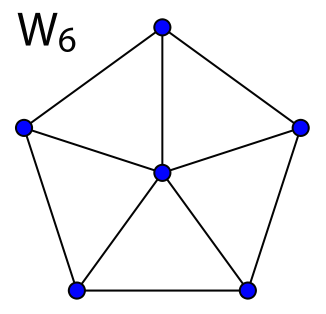
\includegraphics[width=1in]{wheel_graph.png} \]
Show that $W_n$ is always self-dual.
\item Recall that the Petersen graph is
\[ 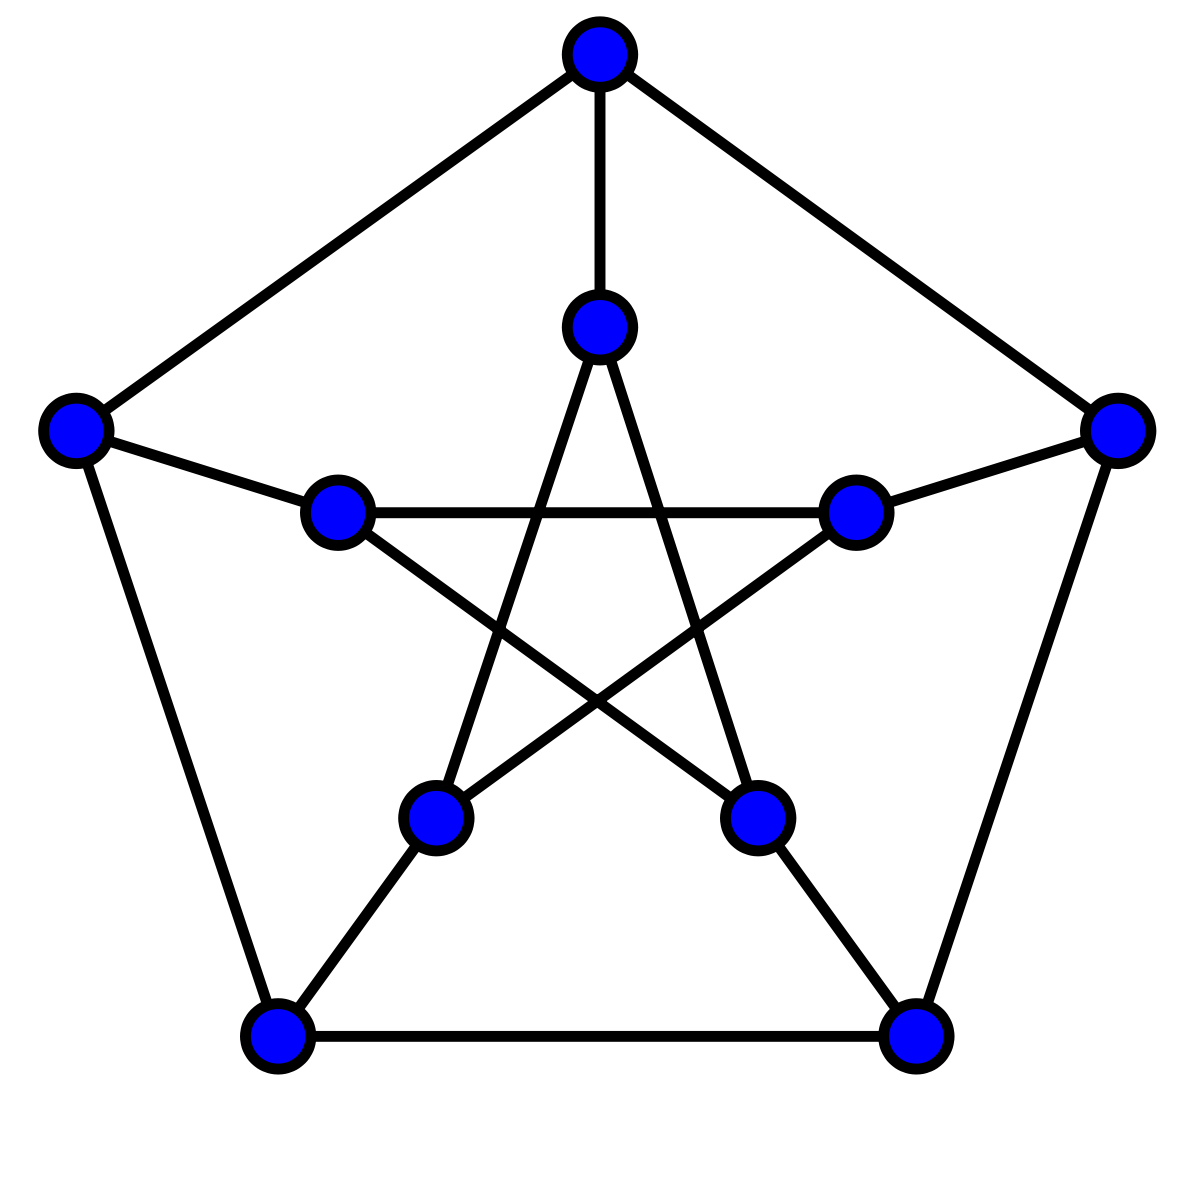
\includegraphics[width=1in]{petersen.png} \]
Find a subgraph of the Petersen graph that's a subdivision of $K_{3,3}$. Conclude that the Petersen graph is not planar. Can you find a subgraph of the Petersen graph that's a subdivision of $K_5$?
\item Show that the planar graphs corresponding to the icosahedron and dodecahedron are dual:
\[ 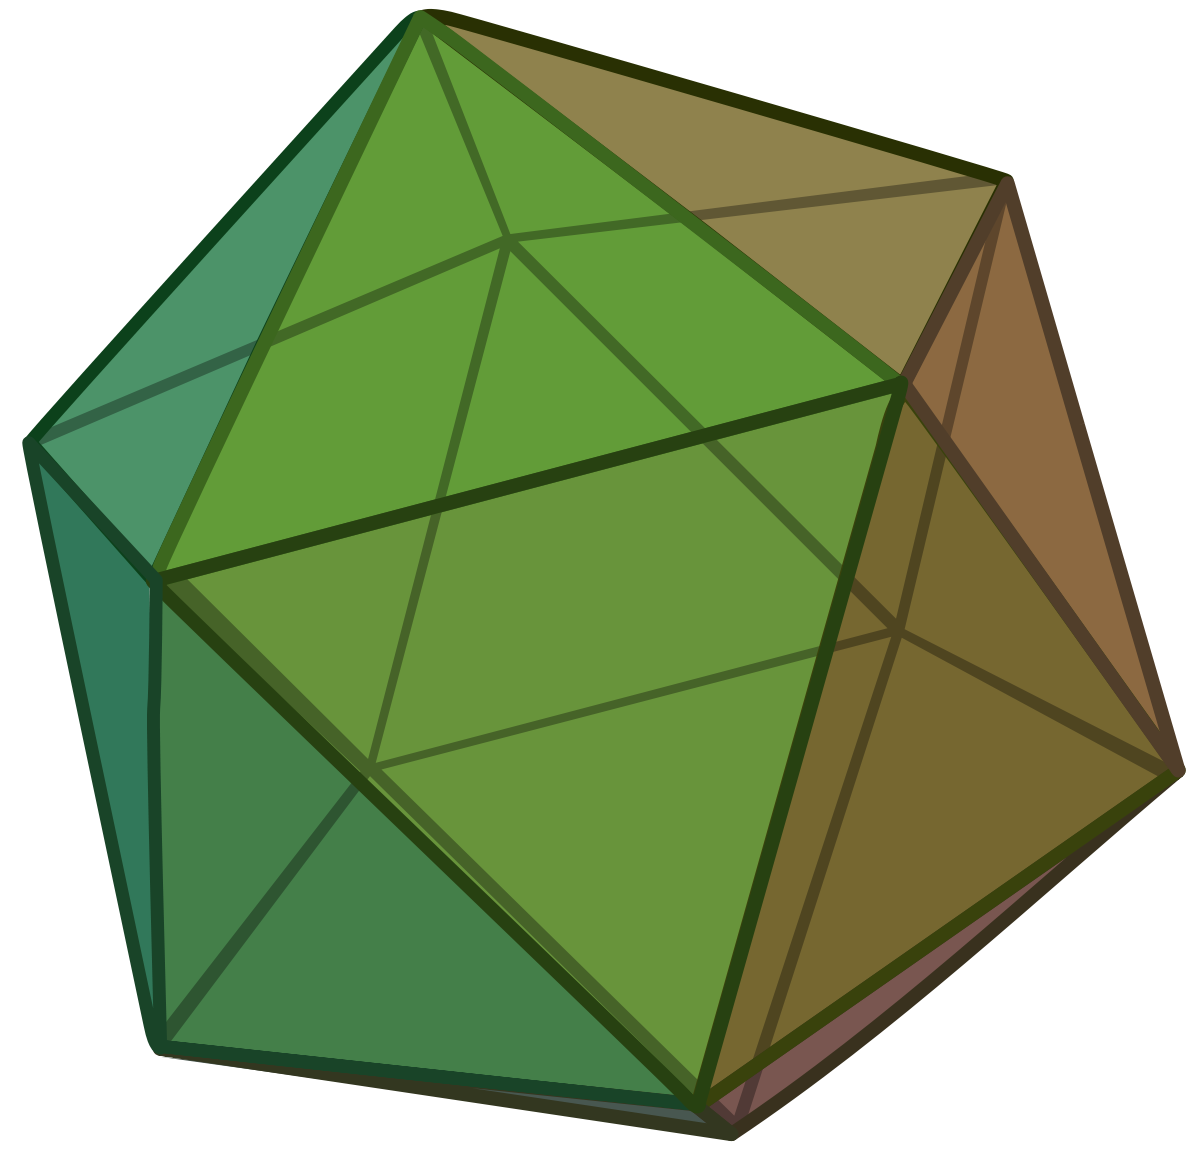
\includegraphics[width=1in]{icosahedron.png} \qquad \qquad \qquad 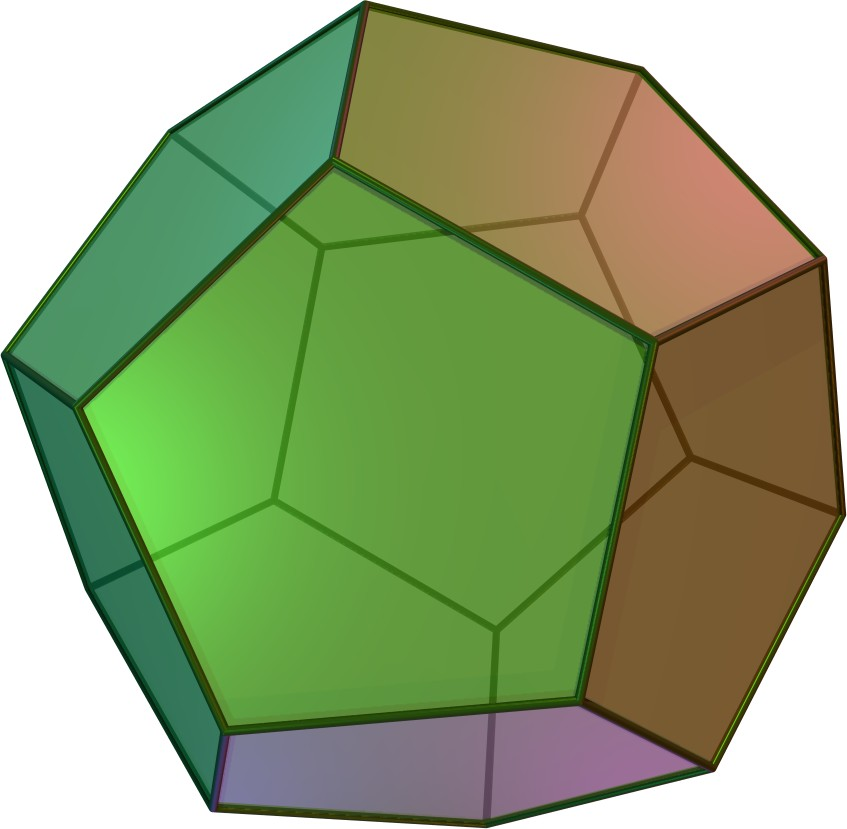
\includegraphics[width=1in]{dodecahedron_solid.png} \]
\end{enumerate}

\end{document}
